\documentclass[12pt]{article}

\usepackage[margin=1in]{geometry}    % Adjusts page margins
\usepackage{graphicx}               % For including images (screenshots)
\usepackage{xcolor}                 % For color usage in listings or text
\usepackage{listings}               % For code listings

\lstset{                            % Settings for the listings environment
	basicstyle=\small\ttfamily,
	columns=fullflexible,
	breaklines=true,
	showstringspaces=false,
	keywordstyle=\color{blue},
	commentstyle=\color{green!50!black},
	stringstyle=\color{red}
}

\title{Week 3 Mini Project Project Documentation}
\author{Jude Eschete}
\date{\today}

\begin{document}
	
	\maketitle
	
	\section{Introduction}
	SymbolBalance is a C++ console application designed to check for balanced symbols in a user-entered expression and convert valid infix expressions into postfix form. It supports parentheses \texttt{()}, braces \texttt{\{\}}, brackets \texttt{[]}, and block comments \texttt{/* */}. The code is organized so that new C++ learners can easily understand the structure and the key algorithms involved.
	
	\section{Design and Pseudocode}
	The primary tasks of this project are:
	\begin{enumerate}
		\item Read the user input.
		\item Check for balanced symbols.
		\item Convert the expression to postfix if symbols are balanced.
	\end{enumerate}
	
	The core data structure used is a stack, which helps match opening and closing symbols. Below is high-level pseudocode for the main tasks:
	
	\begin{lstlisting}[language=C, caption={SymbolBalance Pseudocode}]
		function parseInput():
		read entire line into inputStr
		
		function checkSyntax(inputStr):
		create an empty stack
		for each character (or pair for block comments) in inputStr:
		if opening symbol -> push onto stack
		if closing symbol -> check if top of stack matches
		if mismatch or stack empty -> error
		else pop from stack
		if stack not empty -> error (unclosed opening)
		return success or failure
		
		function postfixExpress(inputStr):
		remove all block comments from inputStr
		remove whitespace
		use an operator stack to convert from infix to postfix
		for each token in the expression:
		if operand -> add to output
		if '(' or '{' or '[' -> push onto stack
			if ')' or '}' or ']' -> pop until matching opening is found
		if operator -> pop from stack while top has >= precedence
		pop remaining operators
		return postfix expression
	\end{lstlisting}
	
	\section{Data Structures}
	\begin{itemize}
		\item \textbf{Stack:} Used to store opening symbols (\texttt{(}, \texttt{\{}, \texttt{[}, \texttt{/*}), and to compare them against closing symbols for validation. Also used for operators when converting infix to postfix.
			\item \textbf{Strings:} Used to capture user input, remove block comments, and build the output postfix expression.
		\end{itemize}
		
		\section{API Specifications}
		\begin{description}
			\item[\texttt{parseInput()}] 
			Prompts the user and reads a complete expression into a member string.
			
			\item[\texttt{checkSyntax()}]
			Validates if the input has balanced symbols. Returns \texttt{true} if balanced, otherwise prints an error and returns \texttt{false}.
			
			\item[\texttt{postfixExpress()}]
			Converts the (already-validated) infix input into a postfix expression. Removes block comments, strips whitespace, and outputs the resulting postfix expression as a string.
		\end{description}
		
		\section{Example Screenshots}
		
		\begin{figure}[ht]
			\centering
			% Replace 'screenshot1.png' with your actual image filename
			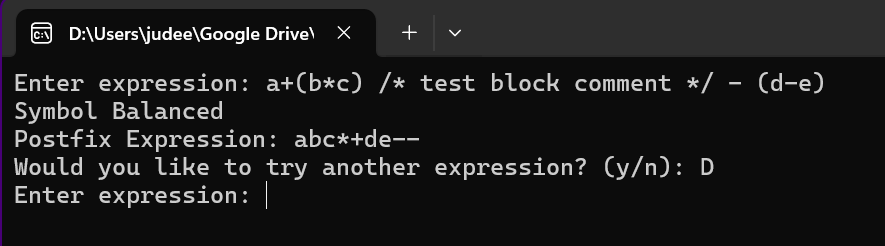
\includegraphics[width=0.9\textwidth]{images/Screenshot_2025-02-17_205622.png}
			\caption{Sample run with balanced parentheses and a comment block.}
			\label{fig:run-balanced}
		\end{figure}
		
		\begin{figure}[ht]
			\centering
			% Replace 'screenshot2.png' with your actual image filename
			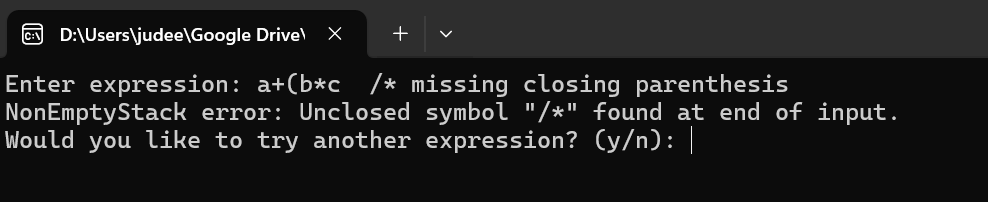
\includegraphics[width=0.9\textwidth]{images/Screenshot_2025-02-17_205741.png}
			\caption{Example of an unbalanced bracket leading to an error message.}
			\label{fig:run-unbalanced}
		\end{figure}
		
		\section{Additional Information}
		\begin{itemize}
			\item The program will prompt you repeatedly for expressions until you choose \texttt{n} or \texttt{N} to exit.
			\item Block comments \texttt{/* ... */} can appear anywhere in the expression; they are treated as opening and closing tokens on the stack.
			\item If a user enters a closing comment without a corresponding opening comment, the program will report an \textit{EmptyStack error}.
			\item The code uses C++ STL features and avoids advanced libraries to maintain simplicity for beginners.
		\end{itemize}
		
	\end{document}
